\section{Referencia de la Clase Informe\-Referencia}
\label{classInformeReferencia}\index{InformeReferencia@{InformeReferencia}}
Genera un informe utilizando una referencia.  


{\tt \#include $<$informereferencia.h$>$}

Diagrama de colaboraci\'{o}n para Informe\-Referencia:\begin{figure}[H]
\begin{center}
\leavevmode
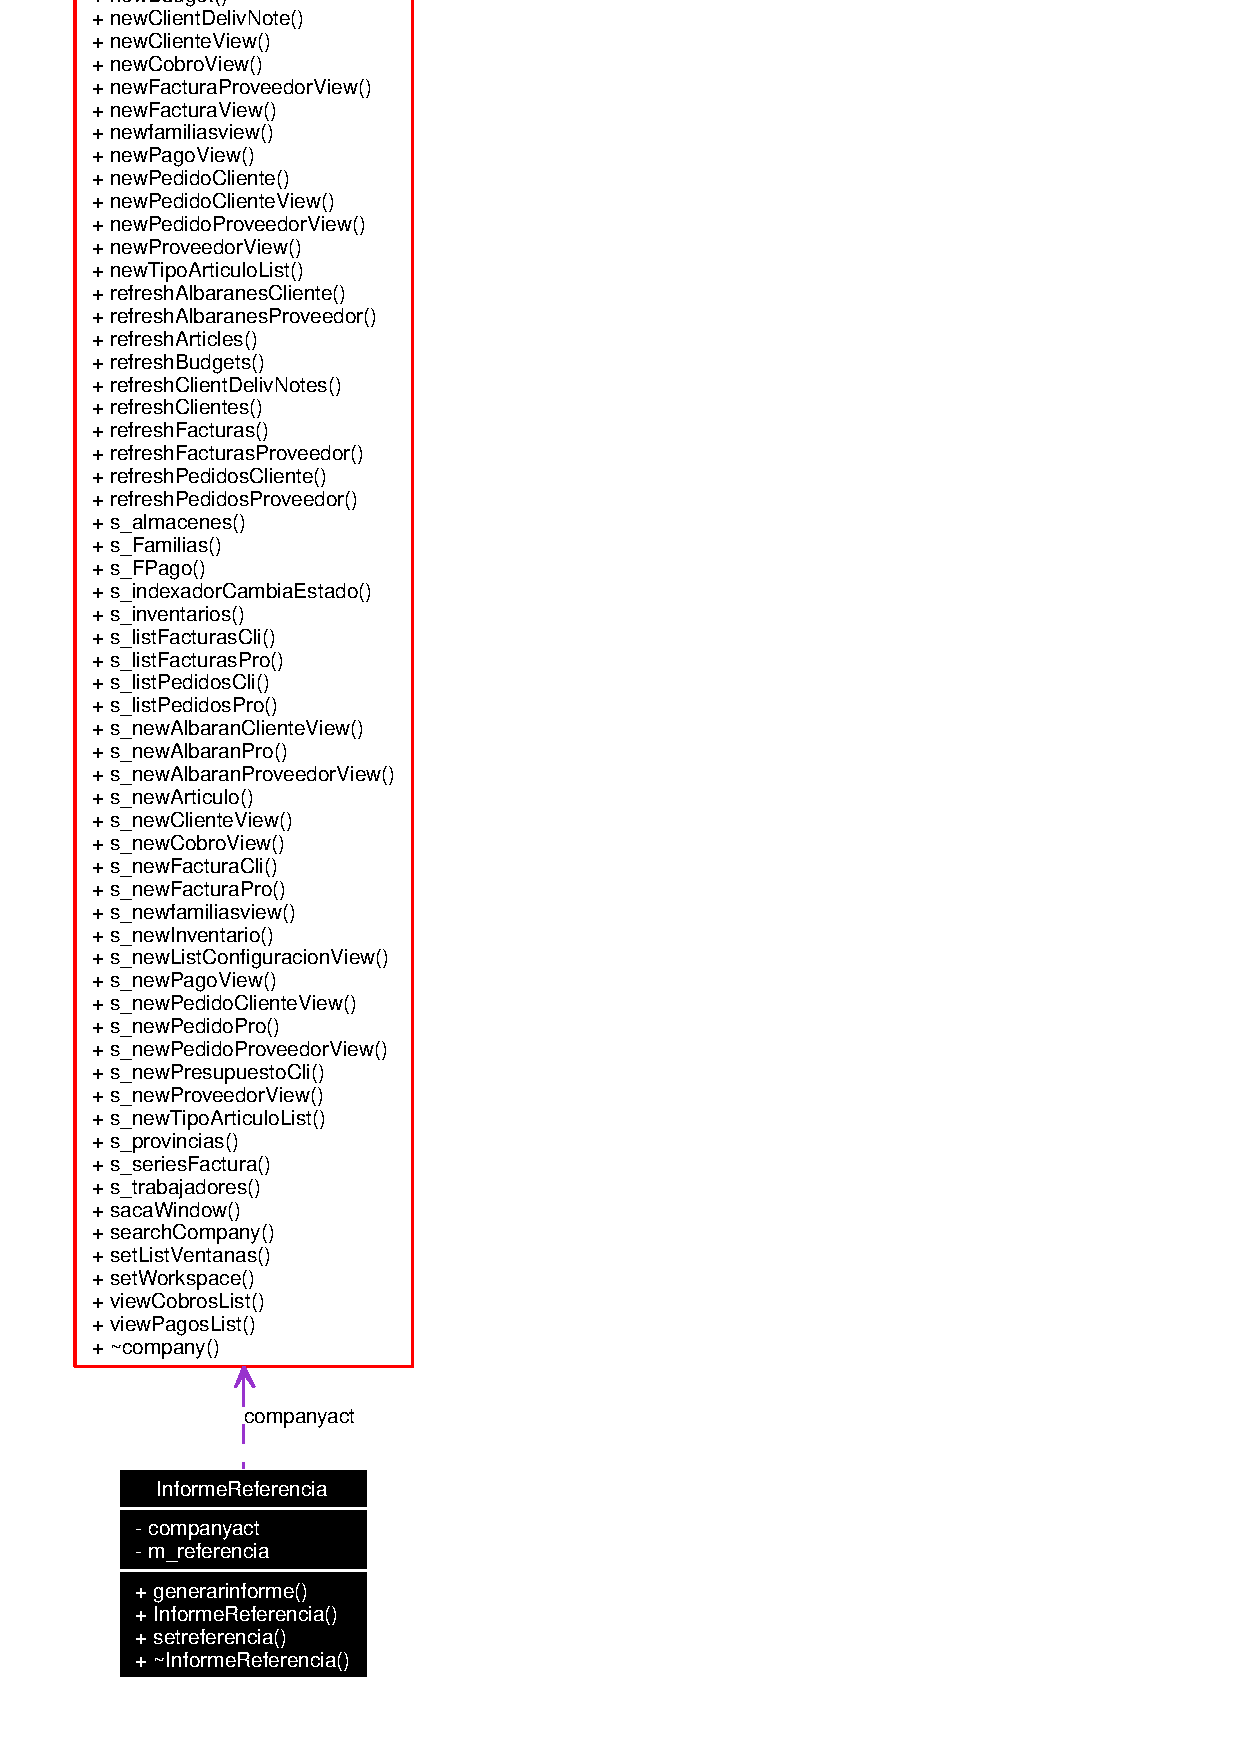
\includegraphics[width=99pt]{classInformeReferencia__coll__graph}
\end{center}
\end{figure}
\subsection*{M\'{e}todos p\'{u}blicos}
\begin{CompactItemize}
\item 
void {\bf generarinforme} ()
\item 
{\bf Informe\-Referencia} ({\bf company} $\ast$)\label{classInformeReferencia_a1}

\item 
void {\bf setreferencia} (QString val)\label{classInformeReferencia_a2}

\end{CompactItemize}


\subsection{Descripci\'{o}n detallada}
Genera un informe utilizando una referencia. 



\subsection{Documentaci\'{o}n de las funciones miembro}
\index{InformeReferencia@{Informe\-Referencia}!generarinforme@{generarinforme}}
\index{generarinforme@{generarinforme}!InformeReferencia@{Informe\-Referencia}}
\subsubsection{\setlength{\rightskip}{0pt plus 5cm}void Informe\-Referencia::generarinforme ()}\label{classInformeReferencia_a0}


Copiamos el archivo.

Copiamos el logo.

Generaci\'{o}n del informe de ventas.

Generaci\'{o}n del informe de compras.

Generacion del informe de totales de ventas.

Calculo de las cantidades totales en moneda.

Total presupuestado.

Total pedido.

Total trabajado.

Total facturado.

Total cobrado.

Generacion del informe de totales de compras.

Calculo de las cantidades totales en moneda.

Total pedido.

Total trabajado.

Total facturado.

Total cobrado. 

La documentaci\'{o}n para esta clase fu\'{e} generada a partir de los siguientes archivos:\begin{CompactItemize}
\item 
informereferencia.h\item 
informereferencia.cpp\end{CompactItemize}
